% Slides accompanying "Learn RISC-V CPU Implementation and BSV" book
% Copyright (c) 2024 Rishiyur S. Nikhil, All Rights Reserved

% -*- mode: fundamental -*-

% Slides accompanying "Learn RISC-V CPU Implementation and BSV" book
% Copyright (c) 2024 Rishiyur S. Nikhil, All Rights Reserved

% This is a preamble shared by all the slide decks

\documentclass[10pt, aspectratio=169]{beamer}

% \documentclass[17pt]{beamer}

% Avail. font sizes: 8pt, 9pt, 10pt, 11pt, 12pt, 14pt, 17pt, 20pt.
% Default font size is 11pt (= 22pt in full screen mode).

\usepackage{verbatim}
\usepackage{fancyvrb}
\usepackage{listings}

% ================================================================
% Themes

\usetheme{Madrid}          % Line at bottom: Author (affiliation), OptTitle, Conf, page 

% \usetheme{Copenhagen}    % Same as Madrid except bottom line: Author, OptTitle

% \usetheme{Berkeley}    % Takes up 1-inch border on left and top

% ----------------
% colorthemes
% (default), beaver, beetle, seahorse, wolverine

\usecolortheme{seahorse}

% ================================================================
% Customization: show table of contents before each section
% Use \AtBeginSubsection    to show before each subsection

% \AtBeginSection[]
% {
%   \begin{frame}
%     \frametitle{Table of Contents}
%     \tableofcontents[currentsection]
%   \end{frame}
% }

% ================================================================

% ----------------
% The bsc compiler and BSV language
\newcommand{\bsc}{\emph{bsc}}
\newcommand{\BSV}{\bf{BSV}}
% ----------------
% ITALICISE WORDS
\newcommand{\ie}{\emph{i.e.,}}
\newcommand{\eg}{\emph{e.g.,}}
\newcommand{\Eg}{\emph{E.g.,}}
\newcommand{\etc}{\emph{etc.}}
\newcommand{\via}{\emph{via}}
\newcommand{\vs}{\emph{vs.}}

% ----------------
% EMPTY BOXES OF VARIOUS WIDTHS, FOR INDENTATION

\newcommand{\hm}{\hspace*{1em}}
\newcommand{\hmm}{\hspace*{2em}}
\newcommand{\hmmm}{\hspace*{3em}}
\newcommand{\hmmmm}{\hspace*{4em}}

% ----------------
% Convenient widths

\newlength{\hlessmm}
\setlength{\hlessmm}{\textwidth}
\addtolength{\hlessmm}{-2em}

\newlength{\hlessmmm}
\setlength{\hlessmmm}{\textwidth}
\addtolength{\hlessmmm}{-3em}

\newlength{\hlessmmmm}
\setlength{\hlessmmmm}{\textwidth}
\addtolength{\hlessmmmm}{-4em}

% ================================================================
% Title page

\title[Learn CPU design \& BSV]{Learn RISC-V CPU Implementation and BSV}

\subtitle{(BSV: a High-Level Hardware Design Language)}

\author[{\copyright} R.S.Nikhil]{Rishiyur S.~Nikhil}
% \institute{Bluespec, Inc.}

% Date is set differently in each slide deck

% \logo{
\includegraphics[height=0.6cm]{../Figures/Bluespec_Logo_2022-10}}

% End of preamble
% ****************************************************************


\date{L15: RISC-V: Fife pipelined CPU: principles}

% ****************************************************************

\begin{document}

% ================================================================

\begin{frame}
 \titlepage

 \begin{center}
  
\includegraphics[height=1cm]{Bluespec_Logo_2022-10}
 \end{center}

\end{frame}

% ================================================================

% -*- mode: fundamental -*-

% ================================================================

\begin{frame}[fragile]
\frametitle{Reminders}

\footnotesize

Please git clone: \url{https://github.com/rsnikhil/Learn_Bluespec_and_RISCV_Design} \\
(git pull for latest version).  Repsitory structure:

\vspace{1ex}

\begin{minipage}{0.5\textwidth}\scriptsize
\begin{Verbatim}[frame=single, numbers=left]
    ./Book_BLang_RISCV.pdf
      Slides/
          Slides_01_Intro.pdf
          Slides_02_ISA.pdf
          ...
      Exercises/
          Ex-03-A-Hello-World/
          Ex-03-B-Top-and-DUT/
          ...
      Code/
          src_Top/
          src_Drum/
          src_Fife/
          src_Common/
          ...
      Doc/Installing_bsc_Verilator_etc.{adoc,html}
\end{Verbatim}
\end{minipage}
\hm
\begin{minipage}{0.45\textwidth}
\begin{itemize}

 \item Slides and Exercise are numbered in sync with book Chapter numbers.

 \item For Exercises, please see Appendix E of the book.  Some (not
       all) exercises have associated code in the {\tt Exercises/}
       directory.

\end{itemize}
\end{minipage}

\vspace{2ex}

To compile and run the code for exercises, Drum and Fife, please make sure you have installed:

\begin{itemize}

 \item \emph{bsc} compiler (see \url{https://github.com/B-Lang-org/bsc})

 \item Verilator compiler (see \url{https://www.verilator.org/})
\end{itemize}

\footnotesize

\end{frame}

% ================================================================

\begin{frame}
\frametitle{Chapter Roadmap}

\footnotesize

\begin{center}
\frame{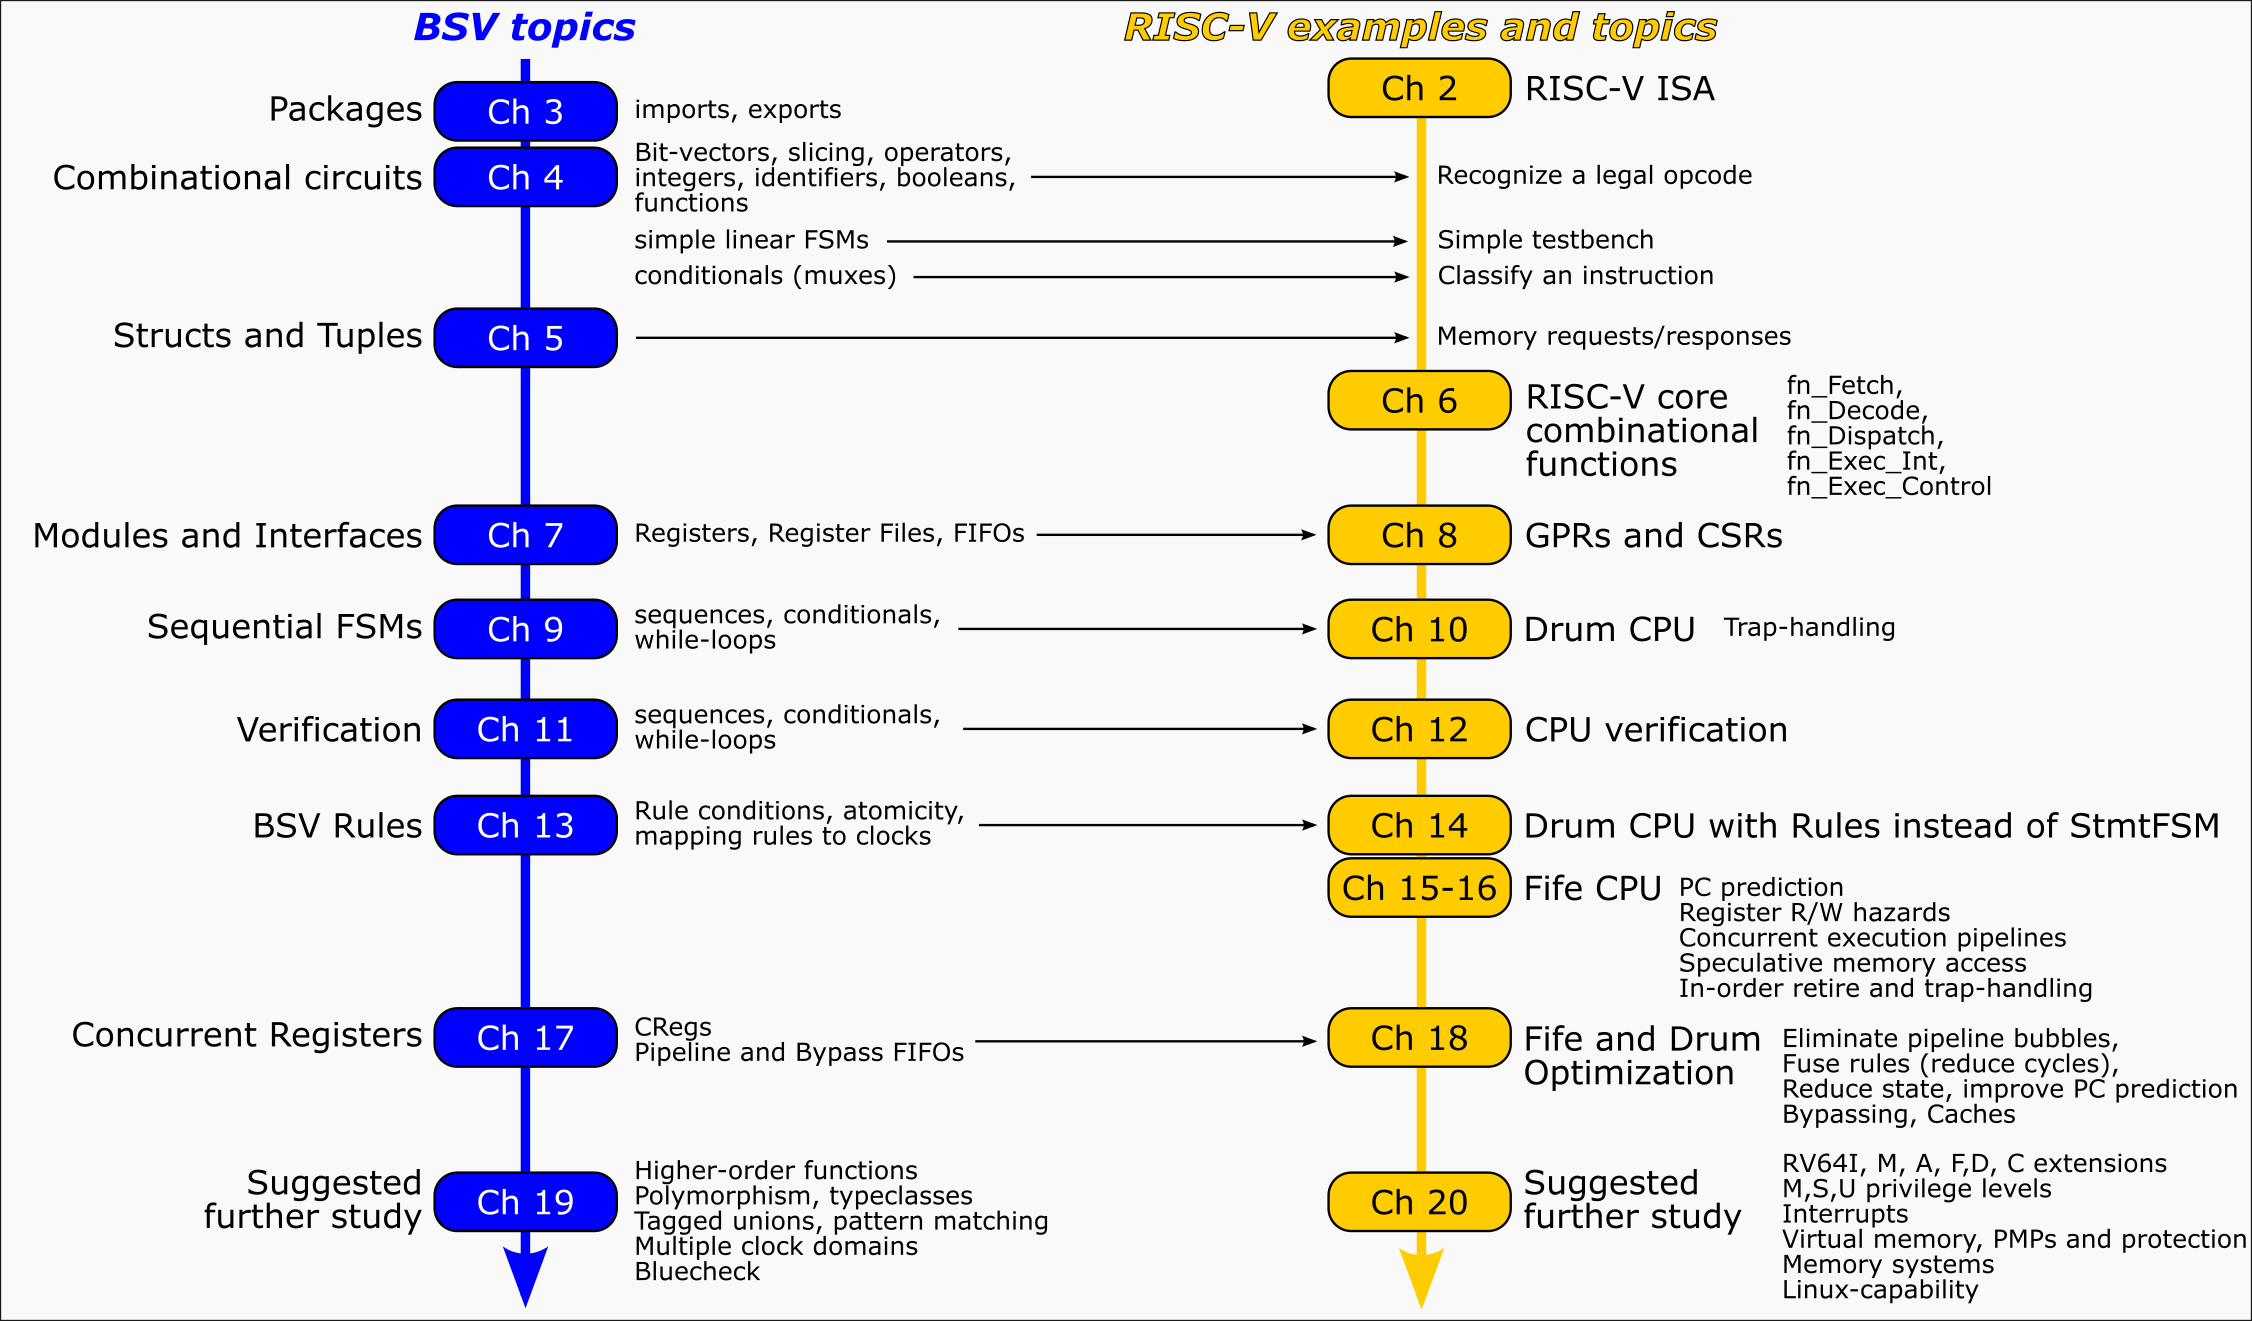
\includegraphics[height=0.825\textheight]{Fig_Chapter_Roadmap}}
\end{center}

\end{frame}

% ================================================================


% ================================================================

\begin{frame}
\frametitle{Table of Contents}

\tableofcontents

\end{frame}

% ****************************************************************

\section{Fife Instruction flow}

\begin{frame}

\begin{center}
  {\LARGE Fife Instruction Flow}
\end{center}

\end{frame}

% ================================================================

\begin{frame}[fragile]
\frametitle{Rules: the fundamental behavioral construct in {\BSV}}

\footnotesize

\begin{center}
 \includegraphics[height=0.6\textheight]{Fig_Instr_Exec_w_FIFOs}
\end{center}

For Fife we interpret each yellow stage as an independent, infinite,
concurrent process.  Each stage repeatedly consumes messages from its
input FIFOs, computes something, and produces messages into its output
FIFOs.

\vspace{1ex}

Thus, multiple instructions may be ``in flight'', each at a different
stage of its processing as it flows down the pipe.

\end{frame}

% ================================================================

\begin{frame}[fragile]
\frametitle{Rules: the fundamental behavioral construct in {\BSV}}

\footnotesize

Pipelining raises four new problems:

\vspace{2ex}

\begin{itemize}

  \item Continuing to Fetch, with PC Prediction and Epochs

  \item Managing Register Read/Write Hazards with a Scoreboard

  \item Retiring outputs of the Execute Stages in Order, with Tags

  \item Allowing Memory Ops to be Pipelined with a Store Buffer

\end{itemize}


\end{frame}

% ****************************************************************

\section{Fife: Continuing to Fetch, with PC Prediction and Epochs}

\begin{frame}

\begin{center}
  {\LARGE Fife: Continuing to Fetch, with PC Prediction and Epochs}
\end{center}

\end{frame}

% ================================================================

\begin{frame}[fragile]
\frametitle{Why do we need PC prediction?  What should we predict?}

\footnotesize

The Fetch stage knows only the current PC, using which it can issue a
read request to memory (IMem) to fetch an instruction.  That
instruction can have several possible outcomes:

\vspace{2ex}

\begin{itemize}

  \item[(T)] It may result in an exception (or be preempted by an external
        interrupt), in which the next PC is taken from CSR {\tt
        mtvec}.

  \item[(B)] It may be a conditional BRANCH instruction; if the branch is
        taken, the next PC is the branch target, otherwise it is PC+4.

  \item[(J)] It may be a JAL/JALR instruction, in which case the next PC is the jump target.

  \item[(F)] (In the most common case) None of the above, in which case the next PC is PC+4 (``fall-through'').

\end{itemize}

\vspace{2ex}

But these outcomes are known only after several cycles, as the instruction flows down the pipe.

\vspace{2ex}

What should the Fetch stage do, in the meantime? \hmm To continue
fetching, it must \emph{predict} (guess) the next PC.

\vspace{2ex}

Since (F) is the most common case, PC+4 is a reasonably good prediction.

\end{frame}

% ================================================================

\begin{frame}[fragile]
\frametitle{What happens when we mispredict?}

\footnotesize

Suppose we mispredict (predict wrong) for instruction $n$.

\vspace{2ex}

Then,

\vspace{2ex}

\begin{itemize}

 \item When we know the correct next-PC for $n$, the Fetch stage must
       be ``\emph{redirected}'' to the correct next-PC from which it
       can resume fetching.

 \item Instructions fetched predictively after $n$ (instructions at
       PC+4, PC+8, ...) and prior to redirection are ``\emph{wrong
       path}'' instructions, and must be discarded.

       \vspace{2ex}

       Equally important: the wrong-paths instructions \emph{should
       not modify architectural state} (registers, CSRs, memory).

\end{itemize}

\end{frame}

% ================================================================

\begin{frame}[fragile]
\frametitle{Using ``epochs'' to manage mispredictions}

\footnotesize

\begin{center}
 \includegraphics[width=\textwidth]{Fig_RISCV_Epochs}
\end{center}

\end{frame}

% ****************************************************************

\section{Fife: Managing Register Read/Write Hazards with a Scoreboard}

\begin{frame}

\begin{center}
  {\LARGE Fife: Managing Register Read/Write Hazards with a Scoreboard}
\end{center}

\end{frame}

% ================================================================

\begin{frame}[fragile]
\frametitle{The problem: Register Read/Write Hazards}

\footnotesize

\begin{itemize}

 \item Consider an instruction I in the Register-Read-and-Dispatch
       stage that needs to read register {\tt x13} (Rs1 or Rs2).

 \item The prior instruction that writes to {\tt x13} may still be in
       the pipeline, ahead of I, in the Execute or Retire stage, and
       may not yet have written to {\tt x13}.

 \item Instruction I must \emph{wait} until {\tt x13} has been
       written, otherwise it will read a wrong (old) value.

\end{itemize}

\vspace{2ex}

This is called a \emph{hazard} or ``race condition''.

\vspace{5ex}

ISA semantics specify that an instruction reads and writes the
architectural state \emph{atomically}.

\vspace{1ex}

But a pipelined implementation may \emph{interleave} the reads and
writes of two instructions unless we take care.

\vspace{5ex}

One solution is to use a \emph{scoreboard}.

\end{frame}

% ================================================================

\begin{frame}[fragile]
\frametitle{Managing Register Read/Write Hazards with a Scoreboard}

\footnotesize

\begin{center}
 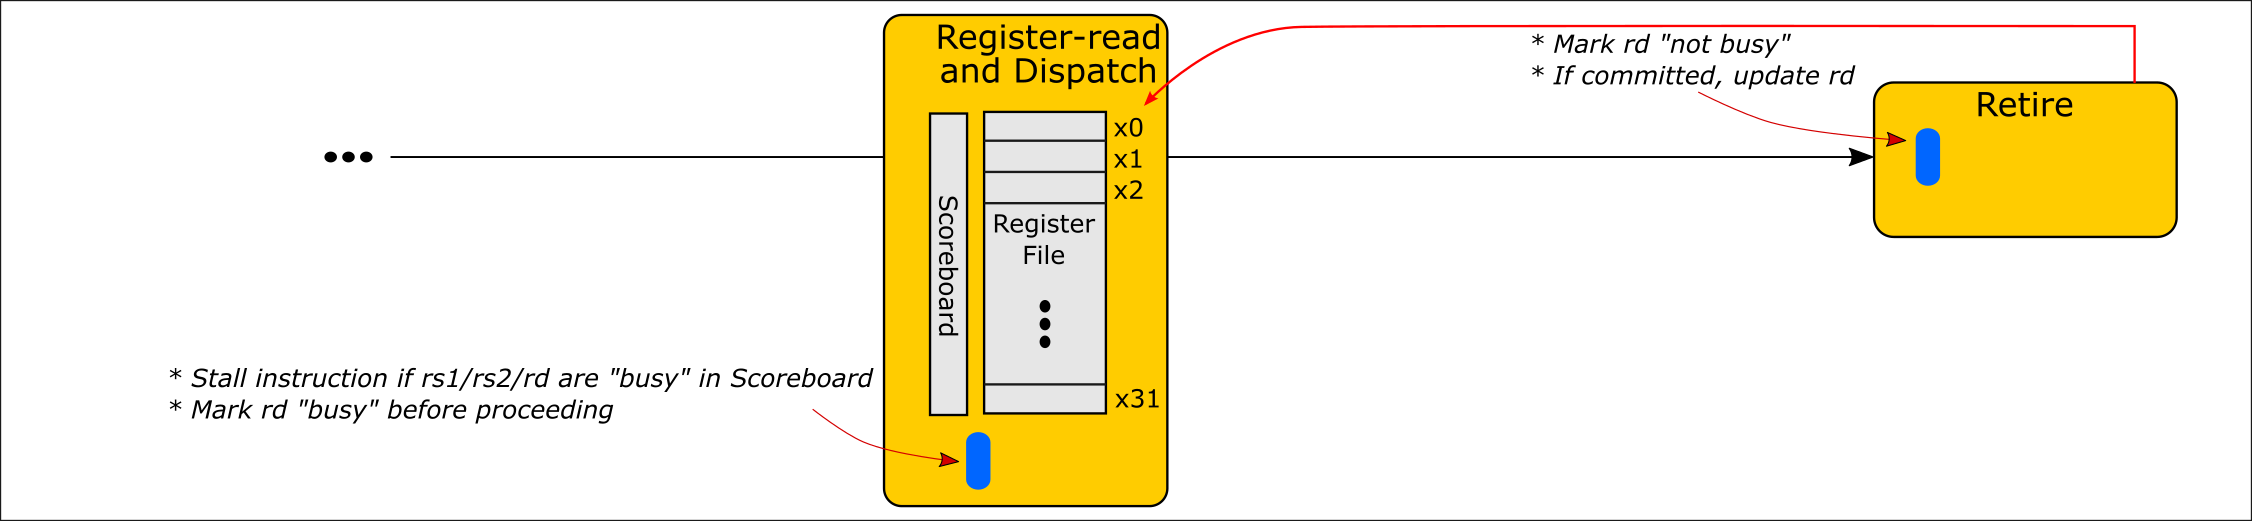
\includegraphics[width=\textwidth]{Fig_RISCV_Scoreboard}
\end{center}

\vspace{2ex}

Note: an instruction's Rd must be restored to ``not busy'' whether the
instruction is committed or discarded.

\end{frame}

% ****************************************************************

\section{Fife: Retiring outputs of the Execute Stages in Order, with Tags}

\begin{frame}

\begin{center}
  {\LARGE Fife: Retiring outputs of the Execute Stages in Order, with Tags}
\end{center}

\end{frame}

% ================================================================

\begin{frame}[fragile]
\frametitle{The problem: varying latencies in Execute pipes}

\footnotesize

\begin{center}
 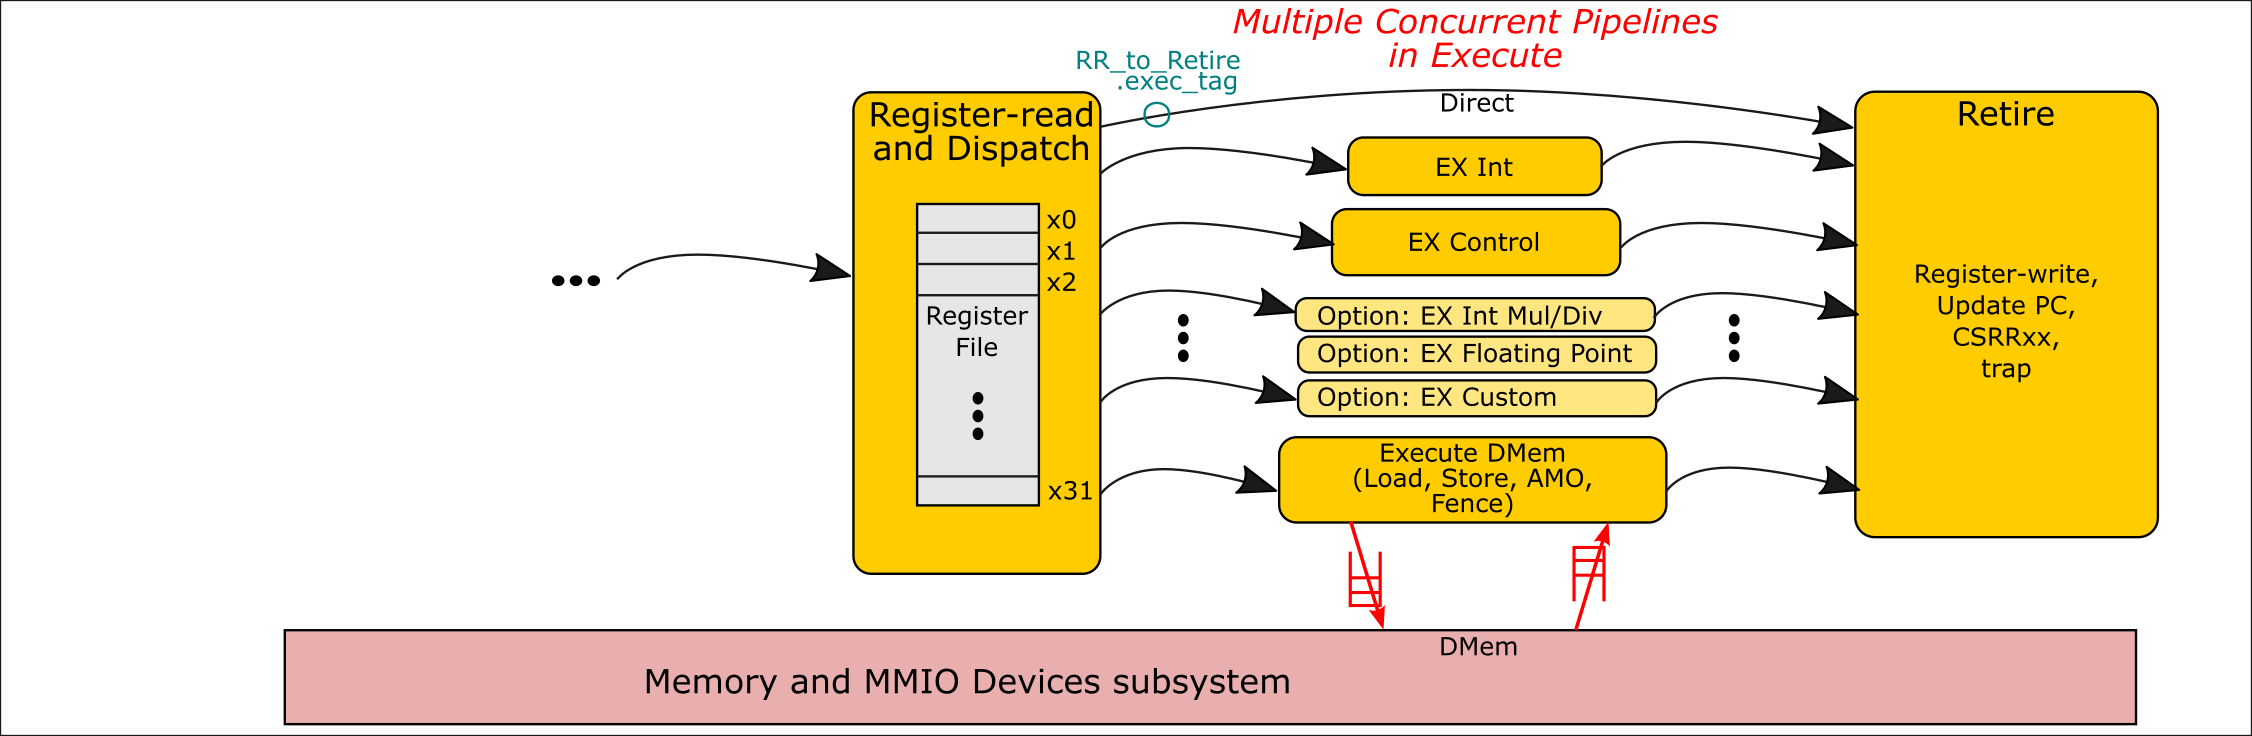
\includegraphics[width=\textwidth]{Fig_RISCV_Retire_Ordering}
\end{center}

\vspace{1ex}

Instructions may not arrive at Retire in the same order that they were Dispatched.

\vspace{1ex}

(In Fife, each pipe is FIFO; but the different pipes may have different latencies.)

\end{frame}

% ================================================================

\begin{frame}[fragile]
\frametitle{Solution: Tags on Direct path}

\footnotesize

\begin{itemize}

 \item In Dispatch, even if an instruction is sent into one of Execute
       pipes, we \emph{also always} send information on the Direct
       path ({\tt RR\_to\_Retire} struct).

 \vspace{1ex}

 \item The {\tt RR\_to\_Retire} struct contains an {\tt exec\_tag}
       field that indicates which Execute pipe (if any) is being used
       for this instruction.

 \vspace{1ex}

 \item The Retire stage observes the {\tt RR\_to\_Retire} struct from
       Direct in order to determine which Execution pipe's output (if
       any) contains the output of the instruction.

       The Retire stage simultaneously dequeues both the FIFO from
       Direct as well as the corresponding FIFO from an Execute pipe.
\end{itemize}

\vspace{1ex}

Thus, if an instruction through an Execute pipe arrives ``early'' at
Retire, it will simply wait there in its FIFO until it is dequeued by
Retire in the correct order.

\vspace{4ex}

{\normalsize \emph{All instructions in the pipelines are considered ``speculative'' until
they are Retired (they may be wrong-path instructions; an instruction
in front of them may trap; or the CPU may take an interrupt).}}

\vspace{1ex}

Side-effects of speculative instructions (register writes, memory
writes) must never be made permanent until they are Retired.

\end{frame}

% ****************************************************************

\section{Fife: Allowing Memory Ops to be Pipelined, with a Store Buffer}

\begin{frame}

\begin{center}
  {\LARGE Fife: Allowing Memory Ops to be Pipelined, with a Store Buffer}
\end{center}

\end{frame}

% ================================================================

\begin{frame}[fragile]
\frametitle{The problem: Speculative memory-writes; speculative MMIO reads and writes}

\footnotesize

\begin{itemize}

 \item Similar to register read-write hazards, we can have memory
       read-write hazards---a STORE instruction may be closely
       followed by a LOAD/STORE instruction for the same (or
       overlapping) memory address.

 \vspace{5ex}

 \item MMIO reads and writes may not be `` memory-like'' at all:

       \begin{itemize}
        \item MMIO reads can have side effects.

        \item After an MMIO write, an MMIO read from that address may
              not return the most-recently--written value.

        \item Two MMIO reads to the same address may not return the
              same value (so, cannot be cached).

        \item Two MMIO writes of the same value to the same address
              cannot be coalesced into one.

       \end{itemize}

       As a result, it is too difficult to perform an MMIO LOAD/STORE
       speculatively; we perform it later, at Retire, when it is no
       longer speculative.

\end{itemize}

\end{frame}

% ================================================================

\begin{frame}[fragile]
\frametitle{Solution: Store Buffer (for non-MMIO accesses)}

\footnotesize

\begin{center}
 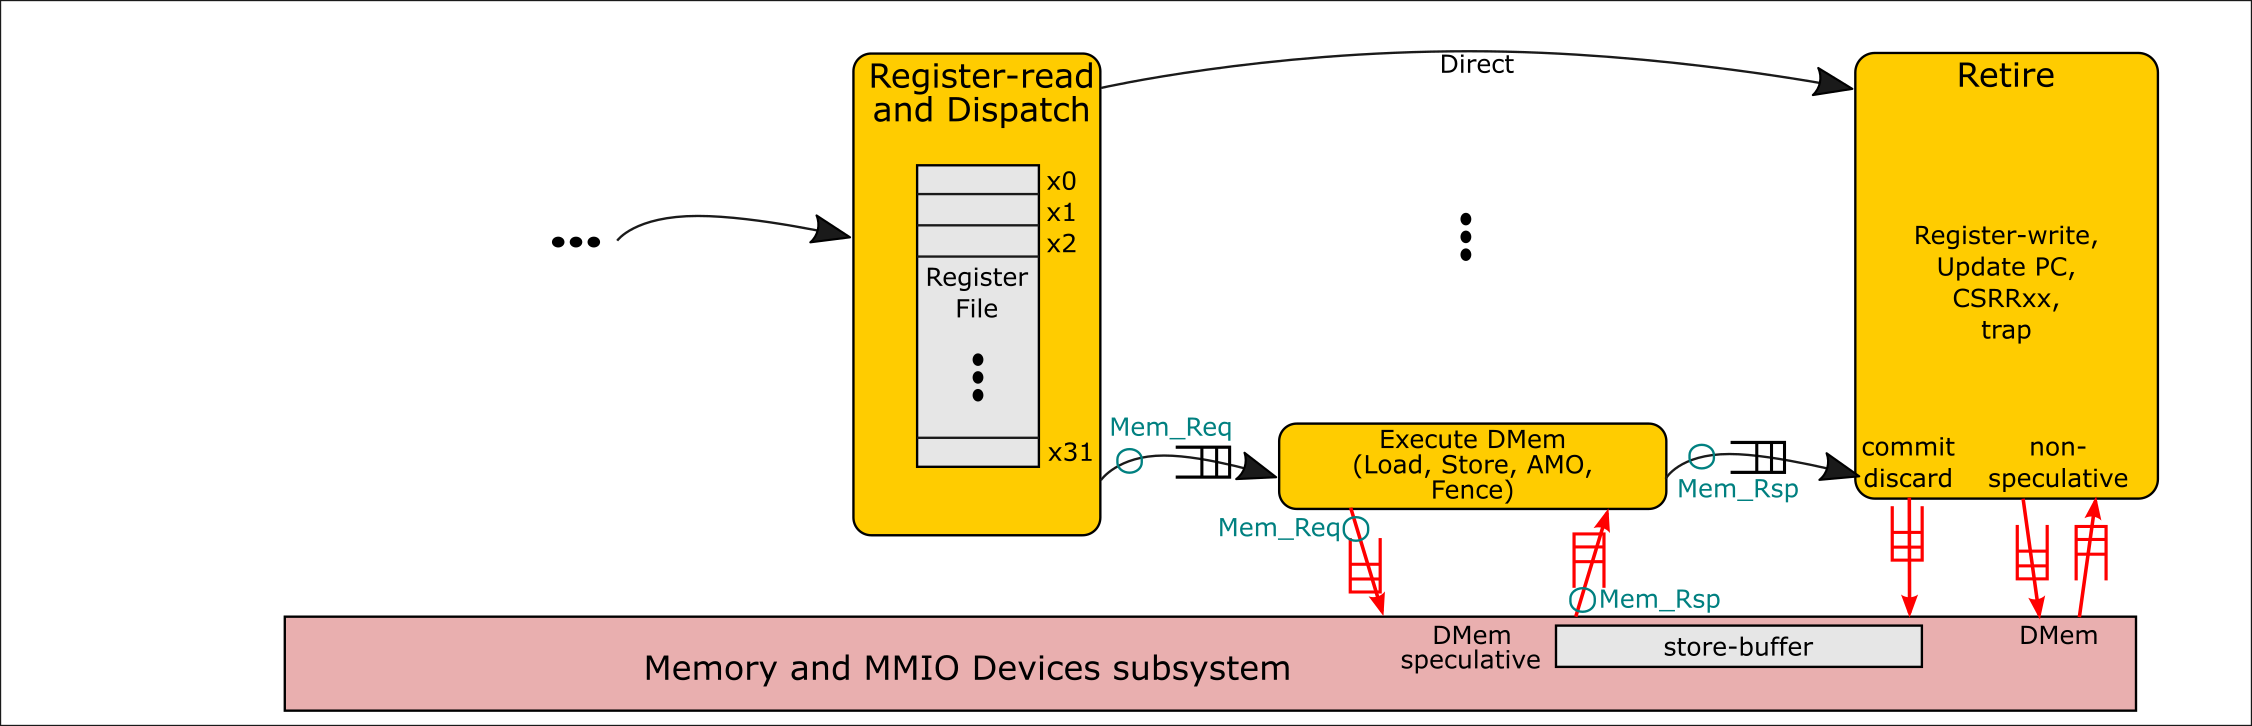
\includegraphics[width=\textwidth]{Fig_RISCV_Store_Buffer}
\end{center}

The \emph{Store Buffer} is a queue of pending non-MMIO STOREs to memory.

\end{frame}

% ================================================================

\begin{frame}[fragile]
\frametitle{Solution: Store Buffer (for non-MMIO accesses)}

\footnotesize

The \emph{Store Buffer} is a queue of pending non-MMIO STOREs to memory.

\vspace{2ex}

In Execute DMem (where everything is still speculative):

\begin{itemize}

  \item A memory (non-MMIO) LOAD first searches the Store Buffer (from
        newest to oldest) in case there were recent STOREs to an
        overlapping address.  For non-overlapping addresses, it
        accesses the memory system as usual.

  \item A memory (non-MMIO) STORE enqueues the stored value into the
        tail of the Store Buffer.

  \item An MMIO LOAD/STORE is \emph{deferred} (returned as-is) in the
        {\tt Mem\_Rsp}.  It will be handled later in Retire.

\end{itemize}

\vspace{2ex}

In Retire:

\begin{itemize}

  \item For a discarded memory (non-MMIO) store, we send a ``discard''
        message to the Store Bufffer; the first item in the Store
        Buffer can be discarded.

  \item For a memory (non-MMIO) STORE, we send a ``commit'' message to
        the Store Buffer; the first item in the Store Buffer can be
        sent into the memory system.

  \item For a discarded MMIO store, we just discard it.

  \item For a deferred MMIO LOAD/STORE, we perform the memory action
        (and handle an ensuing trap, if any).

\end{itemize}

\end{frame}

% ****************************************************************

\section{Fife: Retire stage}

\begin{frame}

\begin{center}
  {\LARGE Fife: Retire stage}
\end{center}

\end{frame}

% ================================================================

\begin{frame}[fragile]
\frametitle{Fife: Retire stage}

\footnotesize

\begin{center}
 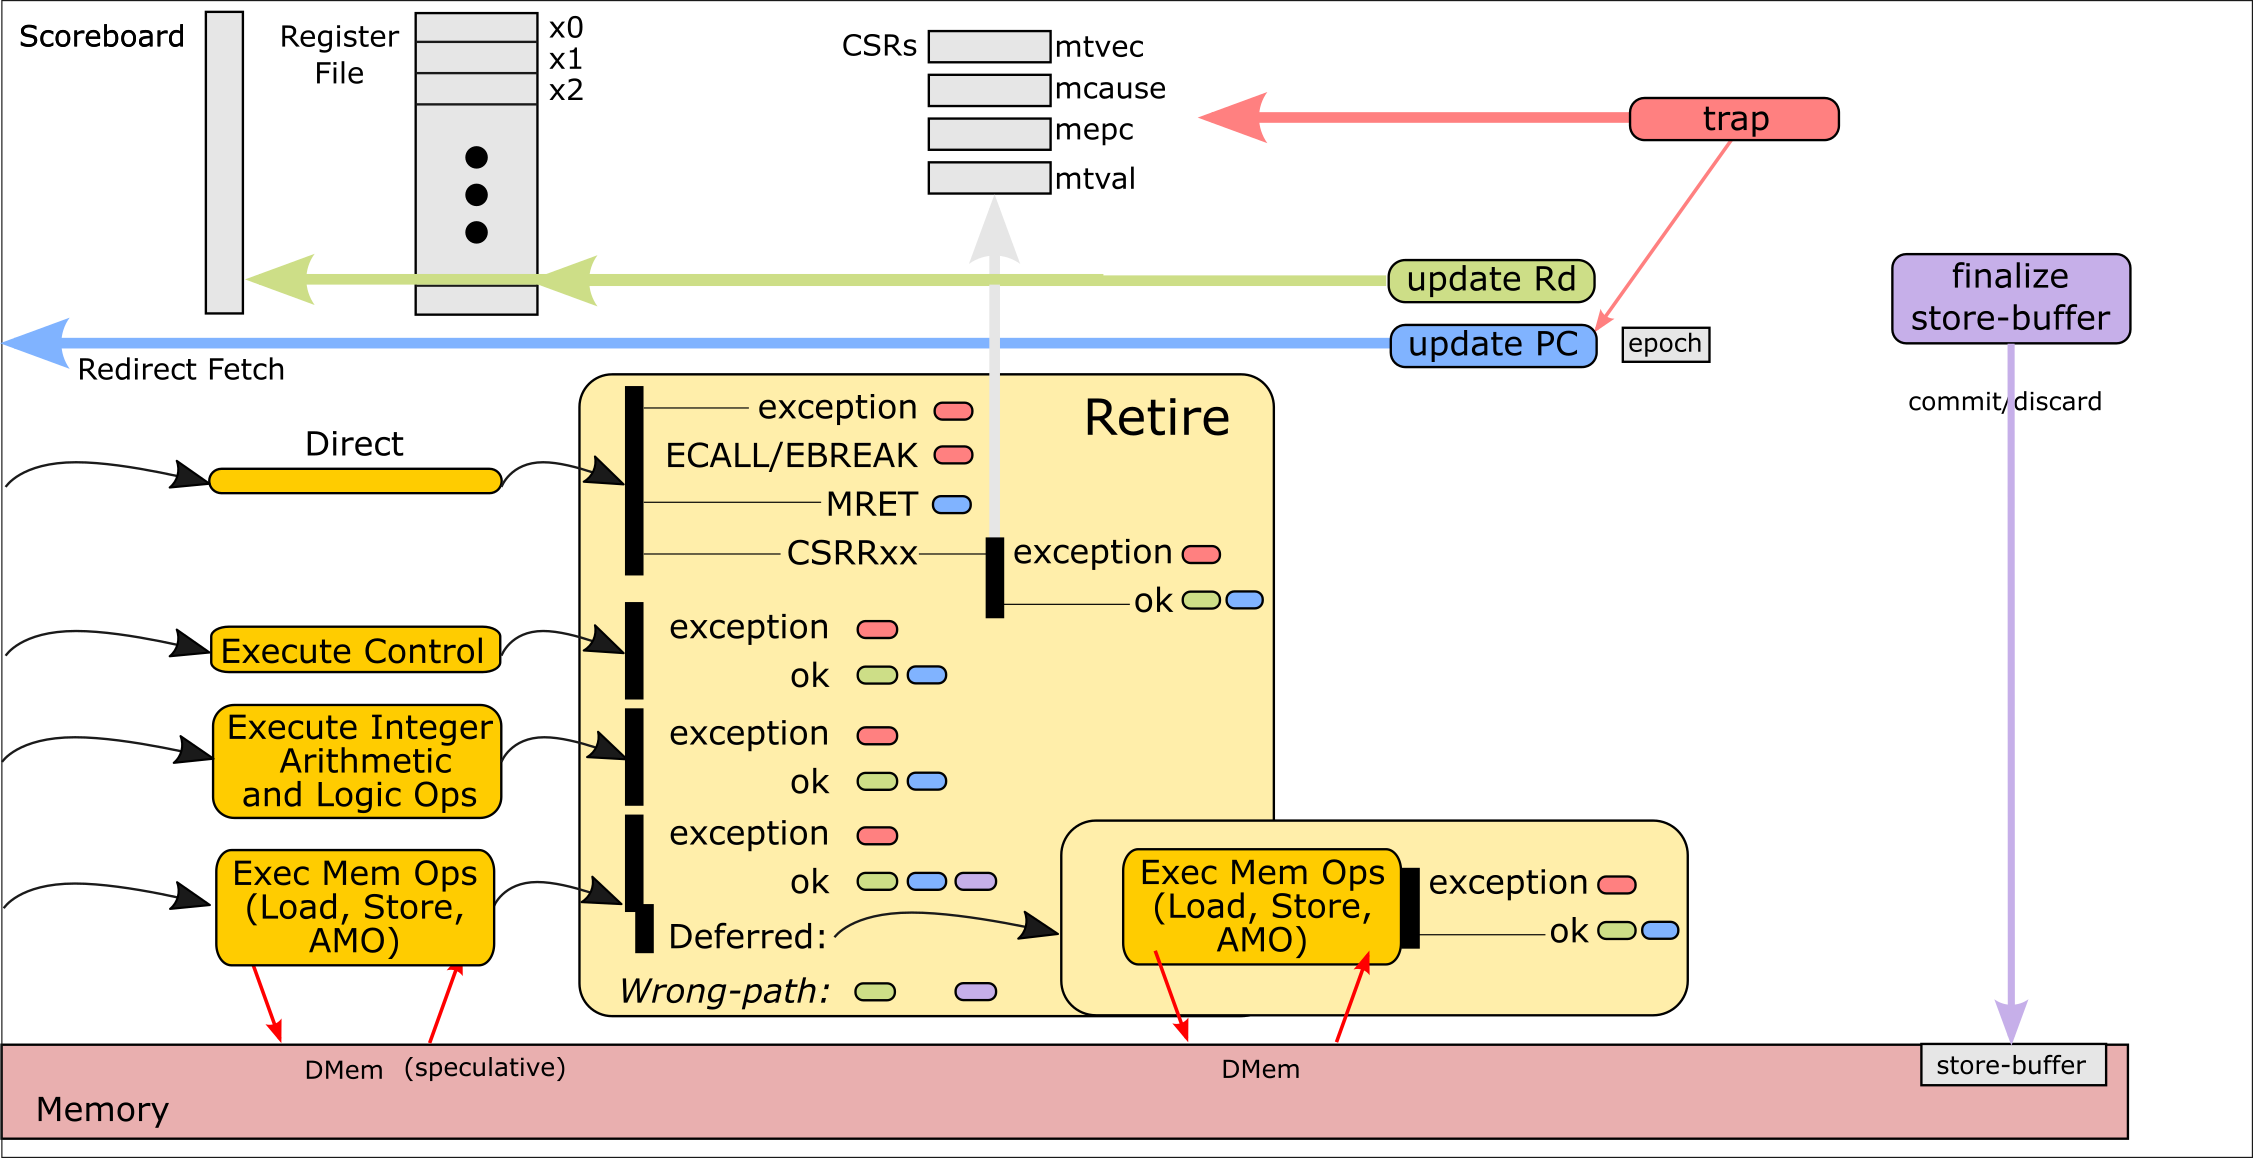
\includegraphics[width=0.8\textwidth]{Fig_Retire_Layers_1_2}

 Similar to Drum, with some differences for prediction/misprediction
 and speculative/non-speculative DMem (next slide).
\end{center}

\end{frame}

% ================================================================

\begin{frame}[fragile]
\frametitle{Fife: Retire stage}

\footnotesize

Differences from Drum:

\vspace{2ex}

\begin{itemize}

 \item ``update PC'' sends a redirect message to Fetch \emph{only} if
       mispredicted.

       On redirect, increment \verb|epoch| and send new epoch with
       redirection.

 \vspace{2ex}

 \item Wrong path: Discard any arriving instruction with the wrong epoch, and:

       \begin{itemize}

        \item If instruction has \verb|Rd|, ``update Rd'' to
              register file should just release reservation, not update Rd.

        \item For memory STOREs (non-deferred), send ``discard''
              message to store buffer.

       \end{itemize}

 \vspace{2ex}

 \item Committed instructions:

       \begin{itemize}

         \item Memory STOREs (non-deferred): send ``commit'' message
               to store buffer.

         \item Non-memory accesses (MMIO, deferred): perform the
               memory access, and handle ensuing traps, if any.

       \end{itemize}

\end{itemize}

\end{frame}

% ****************************************************************

% -*- mode: fundamental -*-

% Slides accompanying "Learn RISC-V CPU Implementation and BSV" book
% Copyright (c) 2024 Rishiyur S. Nikhil, All Rights Reserved

% This is a postamble shared by all the slide decks

% ================================================================

\begin{frame}

\begin{center}
  {\LARGE End}
\end{center}

\end{frame}

% ================================================================


% ****************************************************************

\end{document}
% ****************************************************************
